\setchapterpreamble[u]{\optmargintoc}
\chapter{Particle capture}
\labch{results_particle}

% 0. Cool hook [1 para]
% Hey, if we start off about sensing more generally, we could stick more closely to the original layout?
The ability to sense chemicals was one the earliest kinds of environment sensing to evolve, and chemosensing abilities are known to be present in organisms spanning all biological kingdoms~\sidecite[35pt]{sokolinskaya_molecular_2020}. Humans have chemosensory abilities, most obviously in the forms of a sense of smell and taste, but in myriad other ways such as detecting blood carbon dioxide level~\sidecite[30pt]{cummins_mechanisms_2020}. For certain microorganisms, chemosensing is integral to their ability to swim along chemical gradients to find nutrients (in a process called `chemotaxis')~\sidecite[40pt]{sarvestani_simulation_2016}. Even plants can sense chemicals in their environment, for example to trigger a response to dangerous pathogens~\sidecite[40pt]{zipfel_plant_2014}. Within organisms, chemosensing is everywhere, for example in the form of signalling chemicals that can convey messages between cells. Chemosensing is therefore an incredibly important facet of life as we know it, and in eukaryotes, many of these chemosensors are found on cilia~\sidecite{marshall_cilia_2006}.

% 1. What is chemosensing? [1 para]
% Kind of covered above...

% 2. Why is it important? 
% Kind of covered above...

% 3. Where does it happen? Specific examples, examined more closely? Does chemosensing underpin other senses? Mention GCPRs near the end, and namedrop cilia (INCLUDING MOTILE CILIA) right at the end of this bit, plus motivate a tiny bit as to why one might not be ultra shocked to find them on cilia. [4+ paras]
When the primary cilium was first discovered, it was widely assumed to be useless and vestigial. A sensory role was first proposed for it at the end of the 19th century~\sidecite{zimmermann_beitrage_1898, bloodgood_sensory_2010}, but it took many years for this idea to be taken seriously, whereupon the primary cilium experienced a huge explosion in popularity. More recently, it was realised that motile cilia are also chemosensory, though the evidence has been piling up for a long time~\cite{bloodgood_sensory_2010}.

Primary cilia have a high density of receptors, in particular G-protein-coupled receptors (often shortened to GPCRs)~\sidecite{mykytyn_g-protein-coupled_2017}. G-proteins are a family of proteins found inside cells, that act as molecular switches. The G-protein-coupled receptors are transmembrane structures that bind to a specific extracellular signalling molecule. This binding causes the GPCR to change its shape (i.e. undergo a conformational change) which affects the shape of the intracellular part of the GPCR, which allows this intracellular part to alter the environment within the cilium~\sidecite{mykytyn_g-protein-coupled_2017}, which can in turn affect the cellular behaviour. It is estimated that close to half of all drugs available target these GPCRs~\sidecite{cheng_luciferase_2010}, so understanding ciliary chemoreception is extremely useful.

% \todo{Read tuning into cell's antenna, it's a very good overview of this paragraph}
There are several reasons why primary cilia have a high chemosensor density: the environment very close to the cell is often not a good representation of the actual intercellular medium, because cells have charged lipids on their surfaces that can repel or attract various chemicals and ions~\sidecite{marshall_cilia_2006}. Many cells are also surrounded by a so-called glycocalyx, a several micrometre thick covering of sugars, lipids, proteins~\sidecite{ebong_imaging_2011} that acts as a physical barrier to protect and control entry to the cell, as well as filling various other roles~\sidecite{reitsma_endothelial_2007}; however, this covering will also alter the chemical environment close to the cell~\cite{marshall_cilia_2006}. The no-slip condition on the cell's surface could also mean that the role of advection very close to the cell's surface is almost totally suppressed, thus limiting fluid mixing and therefore chemosensitivity~\cite{marshall_cilia_2006}. There is also the fact that, because the cilium has a very high surface area to volume ratio compared to the rest of the cell, only a small number of chemosensors and signalling molecules are required to create large changes in the concentration of second messengers\boxedsidenote{These are signalling molecules that are released inside cells in response to some extracellular signalling molecule that is detected by a chemosensor on the cell (or `first messengers').} in the cilium's cytoplasm; by comparison, an enormous number of chemosensors would be required to achieve a similar increase~\cite{marshall_cilia_2006}. Our work aims to see if there are further geometric reasons for placing chemosensors on cilia, as well as determining what advantages arise when combing chemosensing with motility.


% 4. Physics bit! Diffusion, Péclet, diffusion limit, electrostatic analogy. Can cilia break diffusion limit? [4+ paras]
\section{Physics of chemoreception}
In 1827, the famous botanist Robert Brown was looking through his microscope at some grains of pollen in water, and noticed that they were jiggling, moving in seemingly random directions with seemingly random speeds~\sidecite{feynman_feynman_2006}. This random motion, eponymously called Brownian motion, was later used by Albert Einstein to prove the existence of atoms. He (correctly) proposed that this random jiggling was caused by the particles that make up the water, moving around and colliding with the pollen grains. At some times the pollen would be bombarded more on one side than another, giving a net force. Since this bombardment is constantly in flux, the direction of pollen motion changes constantly and unpredictably~\sidecite{einstein_uber_1905}. This random motion will eventually cause chemicals to become spread out and mixed: a drop of ink in a glass of water will eventually diffuse to tint the entire glass equally.

At the scale of cells and cilia, this process of diffusion is extremely fast, with a timescale given by
\begin{equation}
    \tau_D = \frac{L_c^2}{D},\label{eq:diffusion_scale}
\end{equation}
for some characteristic length $L_c$. $D$ is the diffusion constant of the molecule being transported. 
For something the size of a small signalling molecule being absorbed by a cilium, this timescale is of the order of $\sim 0.1$ seconds\boxedsidenote{At the synapses between nerve cells, diffusion carries the signal across the gap junction, a distance of a few tens of nanometres \cite{widrow_chapter_2019}. Since human reaction time is only a few hundred milliseconds, this gives an idea of how fast diffusion can happen.}.\nosidecite{widrow_chapter_2019} 


The dominance of advection over diffusion can be quantified by the dimensionless Péclet number:
\begin{equation}
    \mathrm{Pe} = \frac{L_c v_c}{D}\label{eq:def_pe},
\end{equation}
where a large Péclet number means advection is dominant, and vice versa. Humans barely notice diffusion, so for a human this number is incalculably large, but for something like a signalling molecule close to the no-slip boundary of a cell, this number is much smaller than one. The length scale $L_c$ in the expression for the Péclet number, as well as the fact that $D$ tends to be larger for smaller, lighter particles, means that diffusion is an incredibly powerful force at small scales, and is often the dominant factor in molecular transport~\sidecite{berg_physics_1977}.

This leads neatly to the concept of diffusion-limited reactions. If we have some perfectly reactive body with a surface $S$, such that any particle of interest that touches it is immediately absorbed\boxedsidenote{As shown by \citeauthor*{berg_physics_1977}~\cite{berg_physics_1977}, even if chemosensors only cover 1\% of the area of a body, one still has near-perfect absorption, so this is a surprisingly accurate assumption for real systems.}\nosidecite{berg_physics_1977} (or converted to other molecules, or adsorbed, or otherwise removed from the population of particles) then this can be represented as a boundary condition where the concentration of those particles is zero ($c(\left|\mathbf{r}\right|\in S,t)=0$). Far away from this absorbing body, there is some representative unperturbed concentration $c(\left|\mathbf{r}\right|\rightarrow\infty,t)=c_0$. In the steady state, the advection-diffusion equation, which describes the concentration field, is very simply
\begin{equation}
    D \nabla^2 c(\mathbf{r},t) - \mathbf{u}(\mathbf{r},t)\cdot\nabla c(\mathbf{r},t) =  \frac{\partial c(\mathbf{r}, t)}{\partial t} = 0,
\end{equation}
subject to the boundary conditions above, and where $\mathbf{u}$ is the fluid velocity. Fick's law, which relates the concentration gradient to the average particle flux, means that the rate at which this body absorbs particles can be written as
\begin{equation}
    R = \iint_S \mathrm{d}\mathbf{S}\cdot (D\nabla c).
\end{equation}
$R$ is proportional to $c_0$, but we can define a rate constant $k=R/c_0$ which is independent of the far-field concentration.

In the absence of advection, the diffusion equation reduces to
\begin{equation}
    D\nabla^2 c(\mathbf{r}) = 0,
\end{equation}
which is exactly analogous to the source-free Laplace equation for the potential $\phi$ in electrostatics:
\begin{equation}
    \nabla^2 \phi(\mathbf{r}) = 0.
\end{equation}
It is possible to find the concentration field by finding pre-existing solutions for the electrostatic problem in the scientific literature, as electrostatics is a much more widely-studied field. Alternatively, and as shown in the appendix of the article below, one can show that the self-capacitance $C$ of the body can be straightforwardly converted to a rate constant:
\begin{equation}
    k = \frac{D}{\varepsilon_0} C,
\end{equation}
where $\varepsilon_0$ is the dielectric permittivity of free space.
It is relatively straightforward to adapt this for the case of a particle near a no-slip boundary, using the method of images. One can introduce a second equally-charged `image' particle, reflected in the no-slip boundary, and then compute the self-capacitance (and hence reaction rate constant) of the particle in the presence of its image.

This rate of absorption due to pure diffusion is called the diffusion limit, and puts an upper bound on how fast microorganisms and cilia can detect chemicals in the absence of advection. However, microorganisms can swim and cilia can pump fluid. The interesting question, which our work presented in this chapter seeks to answer, is to what extent that additional advection can increase sensitivity. The degree to which a body is breaking the diffusion limit may be quantified by the Sherwood number, defined as the ratio of advective mass transfer to diffusive mass transfer. For the advection-diffusion reaction described above, it could be written in terms of the parameters as:
\begin{equation}
    \mathrm{Sh} = \frac{L_c k}{Dc_0 A} \sim \frac{k}{Dc_0L_c},
\end{equation}
where $A$ is the surface area of the body in question. If $\mathrm{Sh}\ll 1$, there is a strong dominance of diffusion-related mass transfer over advective mass transfer, but once $\mathrm{Sh}\gtrsim 1$, advection begins to dominate. At this point, the advection is sufficient to begin to break the diffusion limit. There is also the analogous Nusselt number (often abbreviated to $\mathrm{Nu}$), which is the equivalent quantity for heat transfer. Since the diffusion equation is identical to the heat equation, there are a lot of helpful similarities between the two problems, and solutions to heat transfer problems can often be straightforwardly transformed to get the solution to the equivalent mass transfer problem.

\section{Our work}
% 5. What did we do? [~10 paras: 1 on what we did, and the rest on the significance of our results]
In our work, we studied the interaction between a chemosensitive cilium and an arbitrary chemical species of interest. We initially assumed that the cilium was perfectly chemosensitive over its entire surface, and would immediately adsorb any signalling molecule that touched it, and that it was attached to a cell that was not itself chemosensitive. Beginning with some analytical calculations that take advantage of the electrostatic analogy, we determined that the elongated shape of the cilium, even in the absence of motility, means it can have a much higher chemosensitivity compared to a flat chemosensitive patch on the cell surface. In a quiescent fluid, for typical cilium dimensions, a chemosensitive cilium is equivalently sensitive to a chemosensitive surface patch with $4\times$ the surface area of the cilium. A more complicated calculation (see the appendix of the article below) revealed that this chemosensitivity advantage is even more pronounced in a shear flow, with the equivalently chemosensitive patch having an area of around $6\times$ the surface area of the cilium. In both cases, we also find that the longer the cilium, the more chemosensitive it becomes, even if we keep its surface area constant. This increase in sensitivity that we have seen purely because of the elongated cilium geometry gives one reason why primary cilia are so often host to chemoreceptors.

\begin{figure}
    \centering
    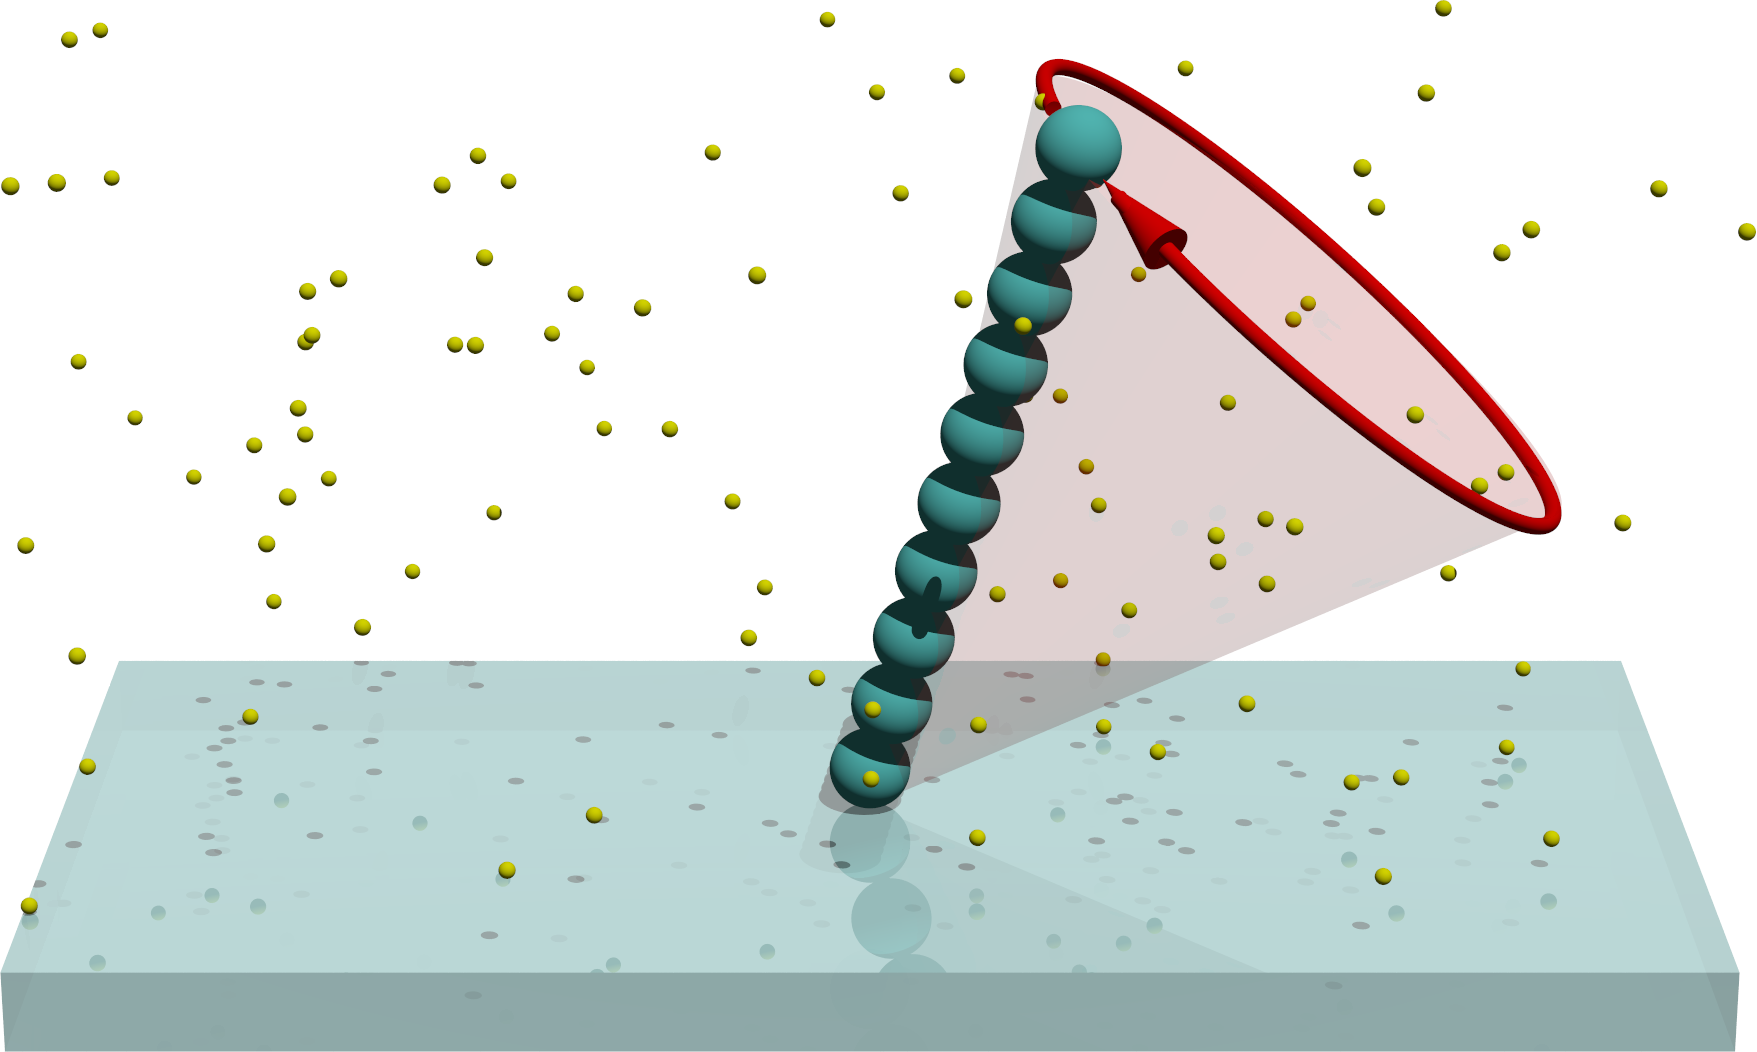
\includegraphics{images_other/absorbing-cilium.png}
    \caption{An illustration of the hydrodynamic simulation. Tracer particles are shown in yellow, and the cilium, simplified to a chain of spheres, is also shown. The trajectory swept out by the cilium is indicated.}
    \label{fig:particle_simulation}
\end{figure}

We then developed a numerical hydrodynamics simulation, wherein individual tracer particles move due to advection and diffusion, and the cilium is approximated by a chain of spheres. The fluid flow due to the motion of these spheres can be computed using superpositions of the Rotne-Prager tensor (Eqs.~(\ref{eq:rp_diag}--\ref{eq:rp_offdiag})), due to the linearity of the Stokes flow. An illustration of the simulation setup is shown in Fig.~\ref{fig:particle_simulation}. 

We used this simulation to understand how much of a gain in chemosensitivity can be achieved by a motile cilium, and found that, provided the cilium beats nonreciprocally in a way that generates a net flow across the cilium, motility can produce a five-fold increase in chemosensitivity compared to a stationary cilium (at realistic cilium Péclet numbers). The increase in chemosensitivity due to cilium motility is even more pronounced than the increase due to cilium geometry, with the chemosensitivity of a motile cilium approaching a factor of $5$ over a stationary cilium at the highest reasonable Péclet numbers a cilium could approach (and hence hugely more sensitive than a chemosensory patch on the cell's surface). At very low Péclet, the cilium barely breaks the diffusion limit, but as the cilium beats faster, the sensitivity rapidly increases. In the high-Péclet regime, the reaction rate scales with $\mathrm{Pe}^{1/3}$, which astoundingly is the same rate that would be found for a sphere in a flow (see box below). The fact that a motile cilium that must pump the fluid itself can reach the same high-Péclet rate scaling as a sphere suspended in a flow is a testament to the efficacy of combining motility with chemosensitivity. This result could go some way to explaining why motile cilia are now known to be chemosensory. The asymmetric beating stroke of the cilium is important, as the net flow it generates is crucial to this increase in chemosensitivity; if a beat is chosen that produces no net flow past the cilium, there is very little increase in chemosensitivity.

\clearpage

\begin{kaobox}[title=Reaction rate for a sphere]
    We can make a scaling argument to derive how the reaction rate $R$ for a sphere in a moving fluid scales with the Péclet number. To begin with, we consider a sphere of radius $a$ in a moving fluid:
    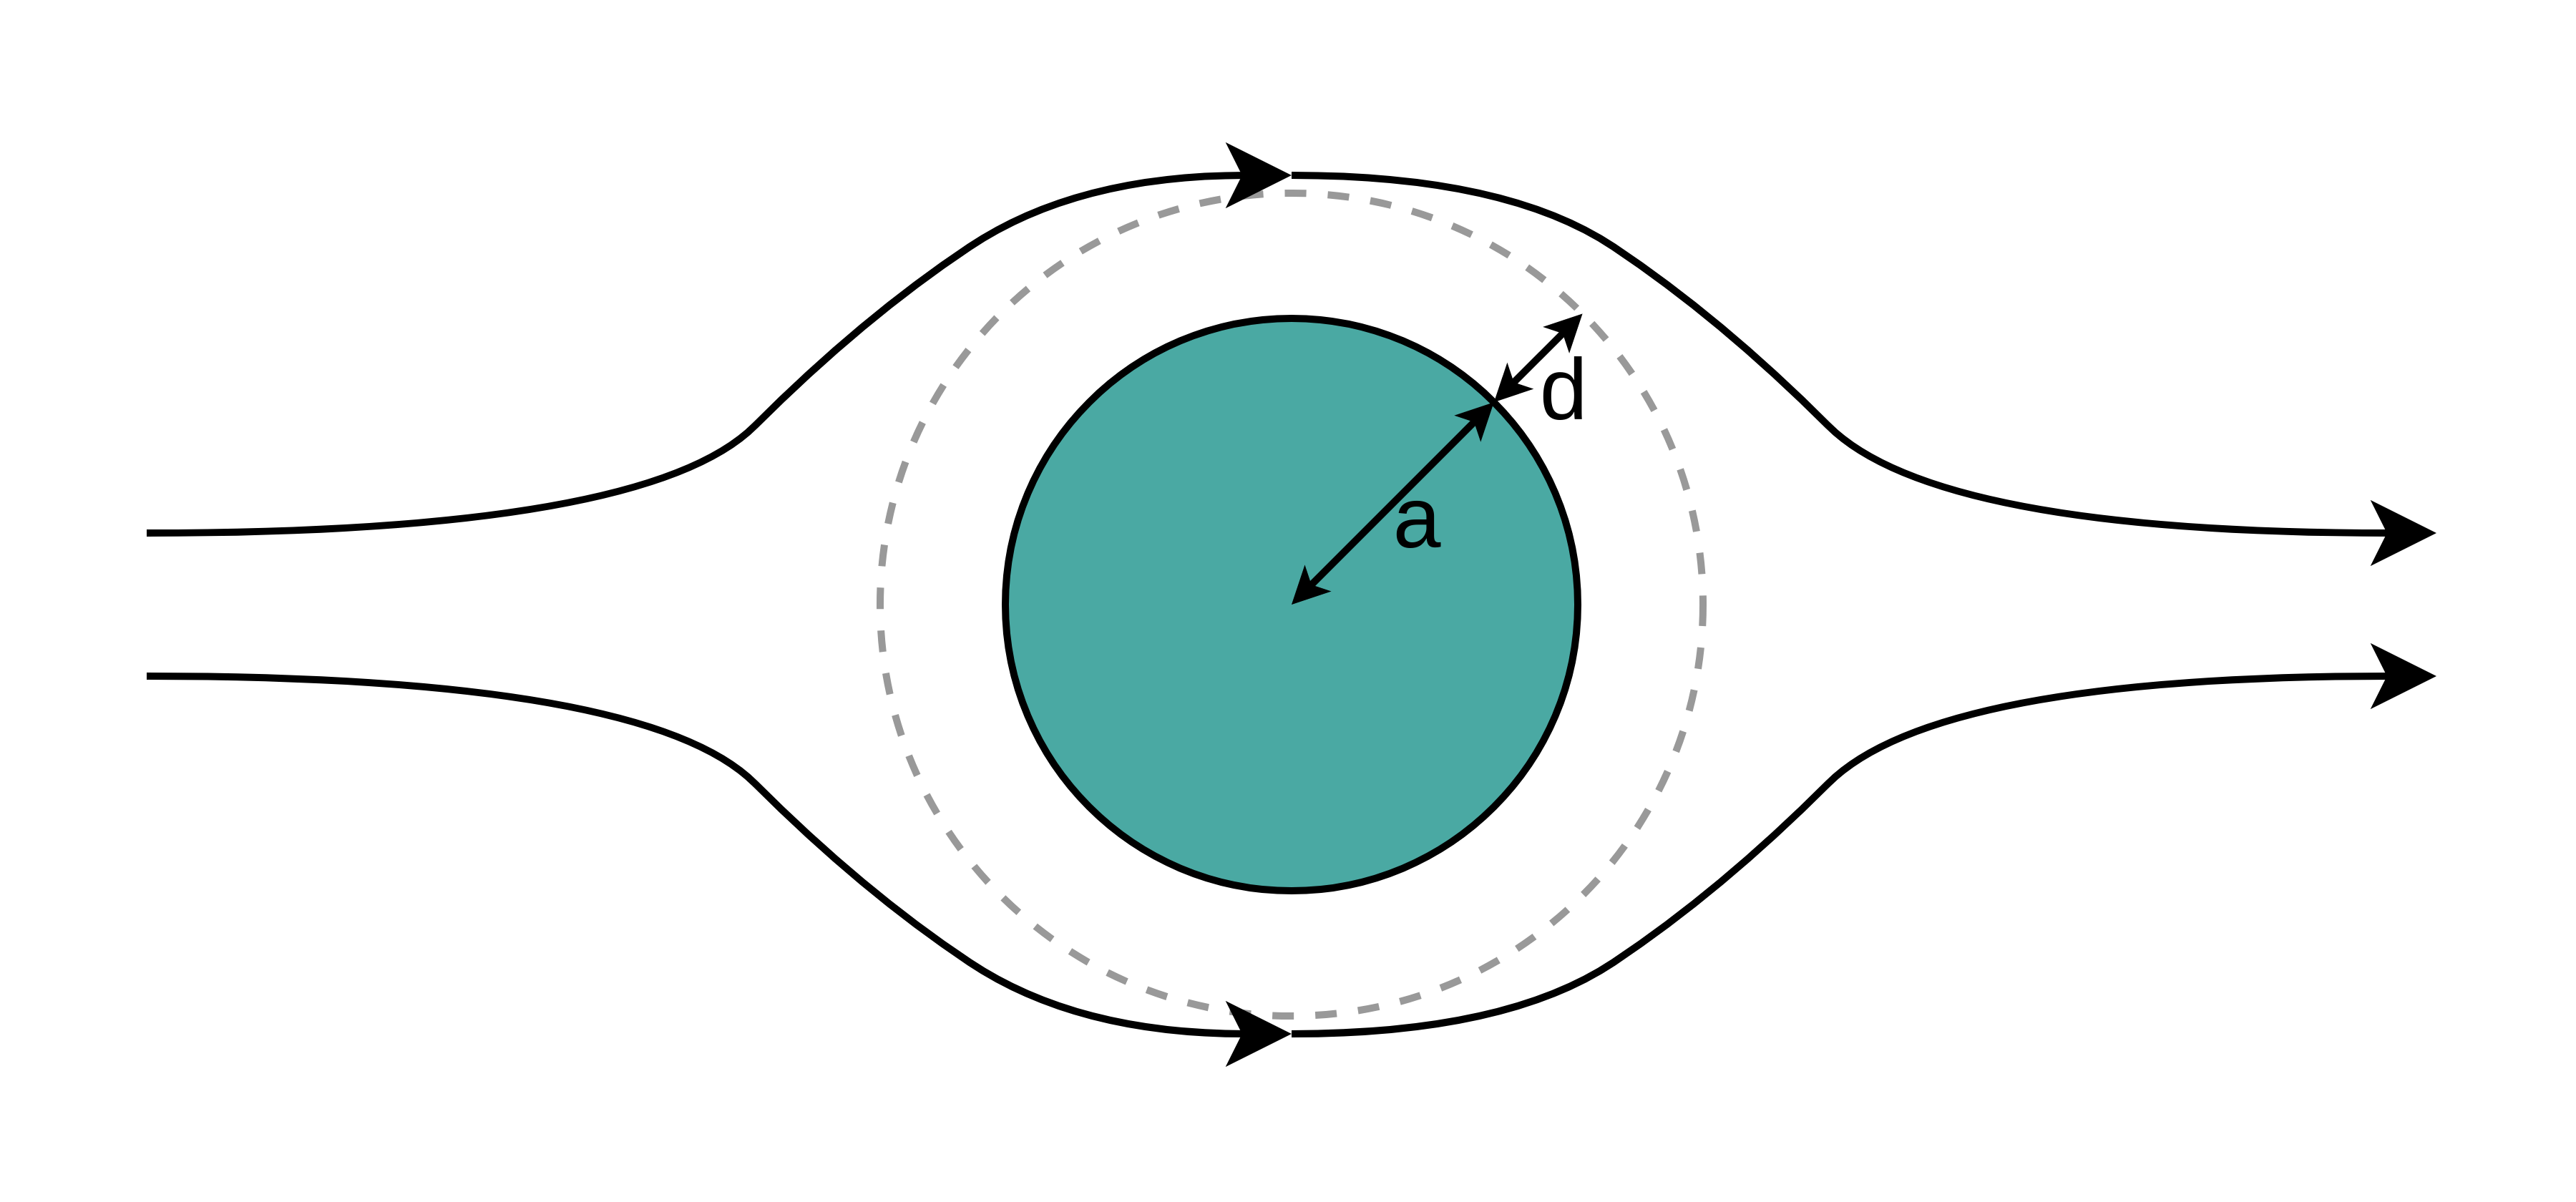
\includegraphics[width=\textwidth]{images_other/sphere_scaling_argument.png}
    We assume that any chemical particles that enter some thin boundary layer of thickness $d$ will make contact with the sphere and be absorbed. Since we know how the diffusion timescale relates to the diffusion length scale (Eq.~\eqref{eq:diffusion_scale}), we know that if the particles take some time $\tau$ to pass the sphere, then
    \begin{equation*}
        d^2 \sim D \tau.
    \end{equation*}
    
    We also know that due to the no-slip condition on the surface of the sphere, the fluid flow very close to the sphere will be well-approximated by a shear flow, and therefore the characteristic flow speed in the boundary layer is $d\dot\gamma$ (where $\dot\gamma$ is the shear rate), which tells us that $\tau \sim 2\pi a/(d\dot\gamma)$.
    
    The reaction rate is then the product of the rate of particle influx ($\sim d\dot\gamma$) with the cross-sectional area of this boundary layer, i.e.
    \begin{equation*}
        R \sim 2\pi a d \cdot d\dot\gamma \sim \left( \frac{a\dot\gamma}{D} \right)^{1/3} = \mathrm{Pe}^{1/3},
    \end{equation*}
    where we have dropped any purely numerical prefactors, as this scaling argument is not nearly precise enough for them to be relevant. Note that we have assumed that $d \ll a$, so that the cross-sectional area of the boundary area can be written as $2\pi ad$; at very high Péclet, this condition is satisfied by definition, so this argument only tells us the scaling behaviour in the high-Péclet limit. Obviously this is an incredibly simplified argument, but much more complicated treatments of the problem give the same result~\cite{bowman_mass_1961}.
    
    It is quite surprising that our results show that a cilium that must pump the fluid itself can reach the same scaling rate as this sphere in a flow, but it is illustrative of just how far motility can increase chemosensitivity.
    
    A similar (albeit more complicated) scaling argument can be made for a cylinder, but due to the Stokes paradox (i.e. there is no well-behaved flow field around a disc in two dimensions at zero Reynolds number) a force density has to be introduced. In this way, a scaling argument can be derived up to a proportionality constant. An approximate value for the proportionality constant had already been found by others~\cite{friedlander_mass_1957}, but we derived an exact value of this constant for the rate per unit length:
    \begin{equation*}
        \frac{dk}{dz} = 3\left(\frac{6}{\pi}\right)^{1/3} \frac{\Gamma(3/4)^{4/3}}{\Gamma(1/3)} D \cdot \mathrm{Pe}^{1/3}.
    \end{equation*}
    The derivation can be found in the appendix of the article below.
\end{kaobox}\nosidecite{bowman_mass_1961, friedlander_mass_1957}

Lastly, we used the same hydrodynamic simulation to investigate the behaviour when placing several chemosensitive motile cilia close together, and found that a bundle motile cilia can be more sensitive together than the same number of individual motile cilia could be apart, i.e. the per-cilium chemosensitivity is higher in a bundle. This result is extremely counter-intuitive, as one would naively expect that many cilia together would all deplete the concentration of signalling molecules and result in a lower per-cilium sensitivity. Instead, every cilium benefits from the fluid flow generated by every other cilium, resulting in the surprising result seen. 



All this shows that by putting chemosensors on cilia, the cell can increase the diffusion limit significantly, and by combining chemosensing with motility, it can break the diffusion limit entirely. This goes some way towards closing some of the open questions introduced in Ch.~\ref{ch:intro}. There are, however, some questions that remain unanswered, which open some possibilities for future work. As previously established, bundles of motile cilia often synchronise, and this work did not examine the impact of metachronal waves on the per-cilium chemosensitivity of a bundle.

There is also potential for a more efficient approach to numerically solving this problem. One consequence of the reciprocal theorem in hydrodynamics is that the particle flux through a surface is invariant under flow reversal, as long as the particle concentration at that surface is uniform~\sidecite{masoud_reciprocal_2019}. If we apply this flow reversal symmetry to the absorption problem, and then apply time-reversal symmetry as well, we have essentially mapped from an absorption problem to an emission problem, where the cilium is now emitting particles but has not changed its trajectory. By inserting and removing particles near the cilium to maintain this concentration, and measuring the flux of particles that escape to infinity, it should be possible to infer the reaction rate. There remain details to be worked out, but it is possible that this approach would increase the efficiency over directly simulating the absorption problem.

% There are some potential applications of this work. For example, very small chemosensors would see an increase in sensitivity if their structure were more cilium-like, or actuated in a way that allows them to move fluid (although progress to date in even making very small chemosensors has been slow~\sidecite{wolfbeis_editorial_2013}, so this application should be considered speculative).

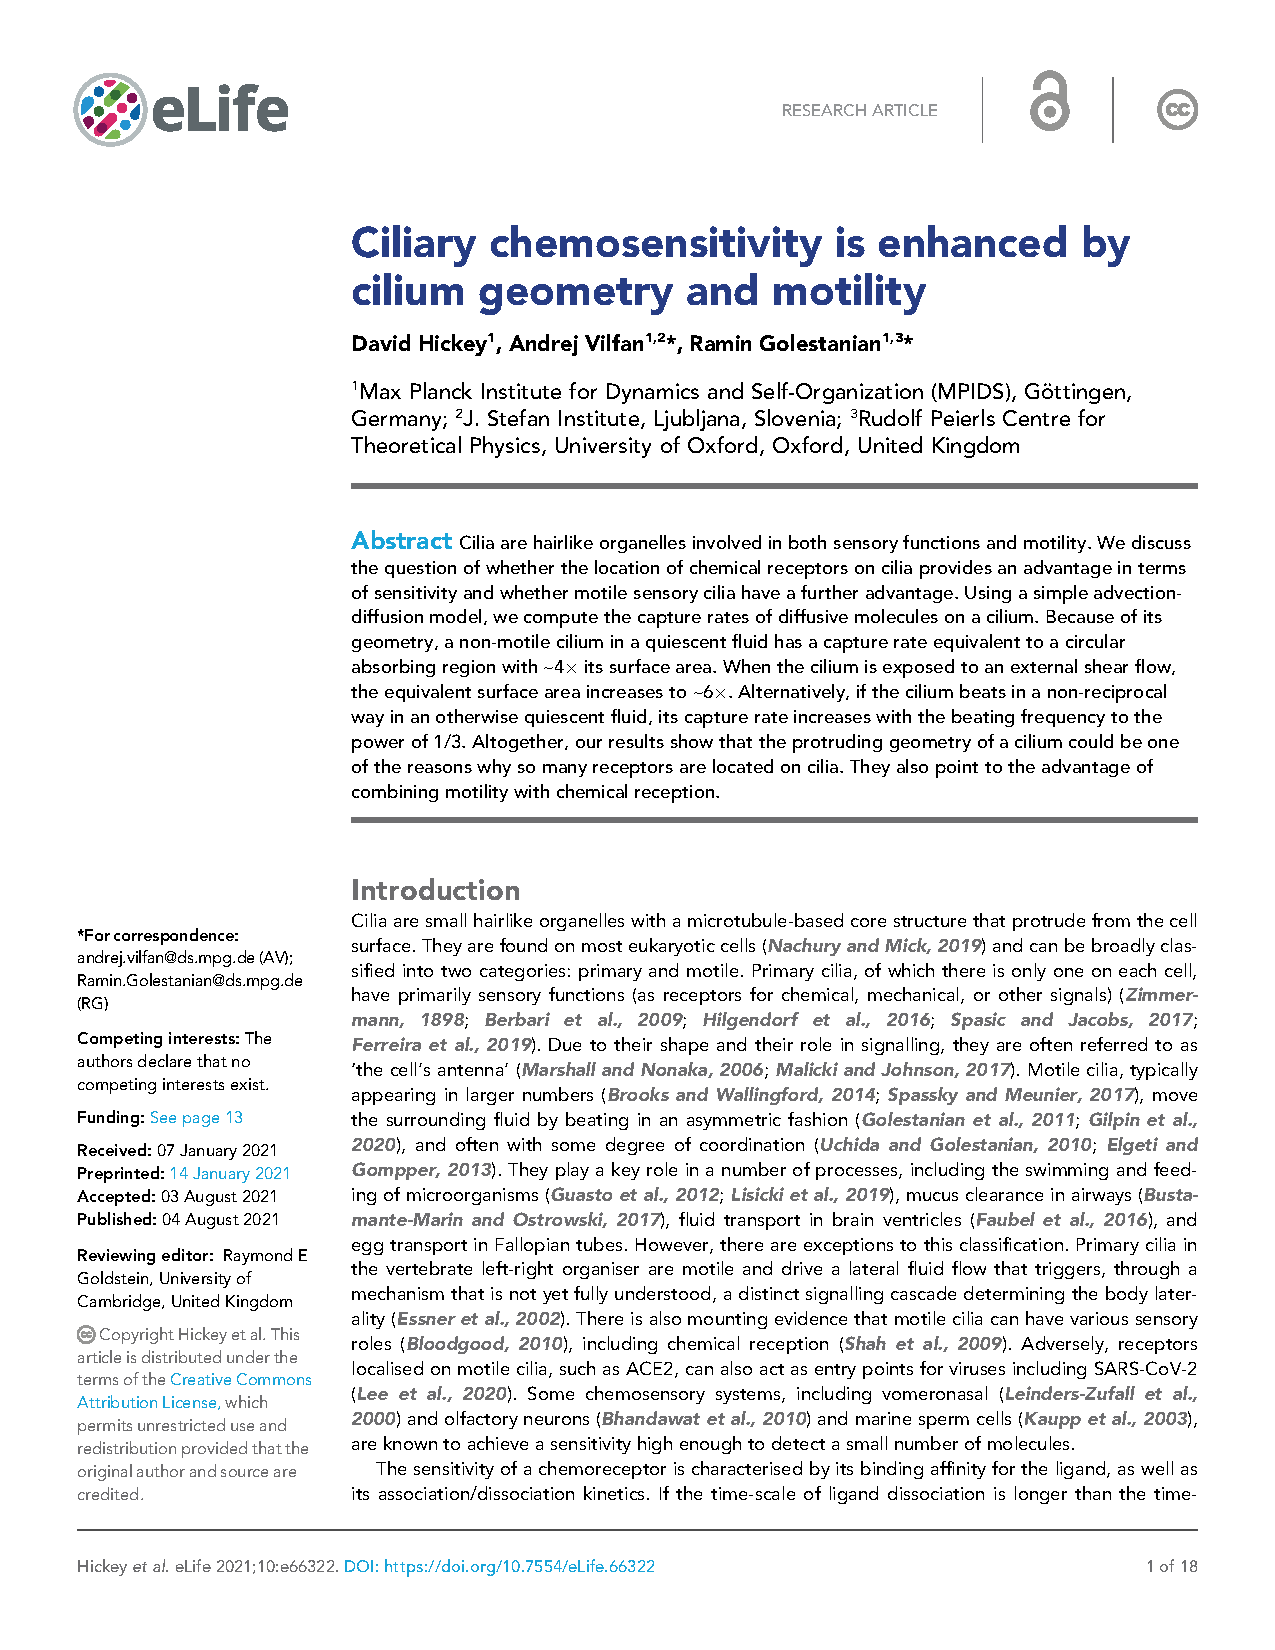
\includepdf[pages=1,pagecommand={ \invisiblesection{Article} \thispagestyle{empty} }]{pdfs/elife-66322-v2.pdf}
\includepdf[pages=2-,pagecommand={ \thispagestyle{empty} }]{pdfs/elife-66322-v2.pdf}

% Now we need a \nocite for every single citation in this paper.
\nocite{nachury_establishing_2019}
\nocite{zimmermann_beitrage_1898, berbari_primary_2009, hilgendorf_primary_2016, spasic_primary_2017, ferreira_cilium_2019}
\nocite{marshall_cilia_2006, malicki_cilium_2017}
\nocite{brooks_multiciliated_2014, spassky_development_2017}
\nocite{golestanian_hydrodynamic_2011, gilpin_multiscale_2020}
\nocite{uchida_generic_2011, elgeti_emergence_2013}
\nocite{guasto_fluid_2012, lisicki_swimming_2019}
\nocite{bustamante-marin_cilia_2017}
\nocite{faubel_cilia-based_2016}
\nocite{essner_conserved_2002}
\nocite{bloodgood_sensory_2010}
\nocite{shah_motile_2009}
\nocite{lee_ace2_2020}
\nocite{leinders-zufall_ultrasensitive_2000}
\nocite{bhandawat_signaling_2010}
\nocite{kaupp_signal_2003}

\nocite{bialek_physical_2005, endres_maximum_2009}
\nocite{berg_physics_1977}
\nocite{adam_reduction_1968}
\nocite{short_flows_2006}

\nocite{marshall_cilia_2006, hilgendorf_primary_2016}
\nocite{marshall_cilia_2006}
\nocite{reiten_motile-cilia-mediated_2017}

\nocite{berg_physics_1977}

\nocite{snow_formulas_1954}

\nocite{challis_olfactory_2015}

\nocite{berg_physics_1977}
\nocite{challis_olfactory_2015, williams_direct_2014}
\nocite{paffuti_results_2018}

\nocite{challis_olfactory_2015}

\nocite{stone_heatmass_1989}

\nocite{bloodgood_sensory_2010}

\nocite{vilfan_generic_2012}

\nocite{smith_fluid_2008}

\nocite{ding_selective_2015, nawroth_motile_2017}

\nocite{berg_physics_1977}

\nocite{frings_single_1990, zhang_ultrasensitive_2013}
\nocite{lai_micro-_2009}

\nocite{ferreira_physical_2017, ferreira_cilium_2019}
\nocite{tanaka_fgf-induced_2005}
\nocite{ding_selective_2015}
\nocite{tripathi_size_2013}
\nocite{nawroth_motile_2017}

\nocite{vilfan_self-assembled_2010, meng_magnetically-actuated_2019, matsunaga_controlling_2019}

\nocite{vilfan_self-assembled_2010}

\nocite{ramirez-piscina_fixed-density_2018}

\nocite{tocino_two-step_2015}

\nocite{berg_physics_1977}

\nocite{masoud_reciprocal_2019}

\nocite{friedlander_mass_1957}
\nocite{vilfan_generic_2012}


\section{Chapter summary}

\begin{itemize}
    \item Chemoreception is an integral part of life, found in all kinds of organisms in all kind of roles, both internal to organisms and externally.
    \item In eukaryotes, a lot of these chemoreceptors are found on cilia. Our work sought to understand some of the reasons why this might be the case.
    \item Our analysis found that all chemoreceptors found on cilia benefit from the geometry of a cilium, which acts to increase their diffusion limit. When a bulk flow is introduced, this geometry-related improvement is even more pronounced.
    \item Motility further increases the chemosensitivity of cilium-bound chemoreceptors. Motile cilia in cilium carpets experience a further increase in per-cilium chemosensitivity over isolated motile cilia, as long as the Péclet number of the beating cilia is high enough.
\end{itemize}
